\section{常用算法}

\subsection{枚举算法}

\begin{frame}
    \frametitle{枚举法的基本思想}
    根据题目的部分条件确定答案的大致范围，并在此范围内对所有可能的情况逐一验证，直到全部情况验证完毕。枚举法也称为穷举法。
    \begin{block}{子数整数问题}
      对于一个五位数$a_1a_2a_3a_4a_5$，可将其拆分为三个子数：sub1、sub2和sub3。

      sub$1=a_1a_2a_3$

      sub$2=a_2a_3a_4$

      sub$3=a_3a_4a_5$

      现在给定一个正整数K，要求求出10000到30000之间所有满足下述条件的五位数，条件是这些五位数的三个子数sub1，sub2，sub3都可被K整除。
    \end{block}
\end{frame}

\begin{frame}
    \frametitle{子数整数问题}
      \begin{minipage}{0.55\linewidth}
            \begin{block}{算法}              
              \begin{enumerate}
                \item n=10000
                \item 对n通过整除和求余运算得到子数
                  \begin{itemize}
                    \item sub1=n//100
                    \item sub2=(n //10) \% 1000
                    \item sub3=n \% 1000
                  \end{itemize}
                \item 判断sub1、sub2、sub3是否都可被K整除。
                \item 如果满足，输出n，n++ ；
                \item 如果不能整除k，n++；
                \item If n<=30000，goto步骤2，else 结束。
              \end{enumerate}
            \end{block}
        \end{minipage}\hfill
        \begin{minipage}{0.43\linewidth}
          \begin{center}
            \begin{tikzpicture}[semithick,node distance=1.5cm,scale=0.5,every node/.style={scale=0.5}]
              \node (start) [startstop] {开始};
              \node (pro1) [op, below of=start] {$n=10000$};
              \node (pro2) [op, below of=pro1,align=center,yshift=-0.5cm] {$sub1=n//100$ \\ $sub2=(n//10) \% 1000$ \\ $sub3=n\% 1000$};
              \node (choice1) [decision, below of=pro2,align=center,yshift=-1cm] {$sub1 \% k ==0 \&$ \\ $sub2 \% k ==0 \&$ \\ $sub3 \% k ==0 $};
              \node (pro3) [op, below of=choice1,yshift=-0.5cm] {输出$n$};
              \node (pro4) [op, below of=pro3] {$n=n+1$};
              \node (choice2) [decision, below of=pro4,align=center] {$n \le 30000$};
              \node (end) [startstop, below of=choice2] {结束};
              \graph[use existing nodes=true]{
                        start  -> pro1 ->  pro2 -> choice1 -> ["Yes",right] pro3 -> pro4 -> (choice2) -> ["Yes",right] end;
                        };
              \draw [->] (choice1)  -| node [above,midway] {No} ++  (4.2,-2.8) -| (pro4);
              \draw [->] (choice2)  -| node [below,midway] {No} ++  (-4.2,8.8) -| (pro2);
          \end{tikzpicture}
          \end{center}
        \end{minipage}
\end{frame}

\begin{frame}[fragile]
    \frametitle{子数整数问题 Python代码}
\begin{codeblock}{子数整数问题}
k = int(input("请输入k："))
for value in range(10000, 30001):
    sub1 = value // 100
    sub2 = value // 10 % 1000
    sub3 = value % 1000
    if sub1 % k == 0 and sub2 % k == 0 and sub3 % k == 0:
        print(value)
\end{codeblock}
\end{frame}

\begin{frame}
    \frametitle{枚举算法的特点}
    \begin{itemize}
      \item 枚举法是一种几乎什么问题都能解决的一般性方法。
      \item 简单粗暴，他暴力的枚举所有可能。
      \item 效率低下，但是可用枚举法求解一些小规模的问题实例。
      \item 如果解决问题实例不多，而枚举法可用一种可接受的速度对问题求解，那么花时间去设计一个更高效的算法是得不偿失的。
    \end{itemize}
\end{frame}

\subsection{迭代算法}

\begin{frame}[fragile]
    \frametitle{迭代算法}
    迭代法也称为“辗转法”，是一种不断用变量的旧值推算出新值的方法。

    迭代算法是用计算机解决问题的一种基本方法，它利用计算机运算速度快、适合做重复性操作的特点，让计算机对一组指令(或一定步骤)进行重复执行，在每次执行这组指令(或这些步骤)时，都从变量的原值推出它的一个新值。

\begin{codeblock}{求1到100的和}
  i = 0
  sum = 0
  while i < 101:
      sum = sum + i
      i = i + 1
\end{codeblock}
    
\end{frame}

\begin{frame}[fragile]
    \frametitle{迭代算法验证谷角猜想}
      日本数学家谷角静夫在研究自然数时发现了一个奇怪现象：对于任意一个自然数n，若n为偶数，则将其除以2；若n为奇数，则将其乘以3，然后再加1。如此经过有限次运算后，总可以得到自然数1。
      \bigskip

      \begin{minipage}{0.53\linewidth}
            算法分析：
            \begin{enumerate}
              \item 确定迭代变量，n就是迭代变量；
              \item 确定迭代关系，有两种迭代关系：一种是当n为偶数时n=n/2，一种是当n为奇数时n=n*3+1；
              \item 迭代控制，通常就是找到循环结束条件，本例就是当n=1结束，验证猜想成功。
            \end{enumerate}
        \end{minipage}\hfill
        \begin{minipage}{0.43\linewidth}

\begin{codeblock}{迭代法验证谷角猜想}
  n = int(input("请输入n："))
  while n != 1:
      if n % 2 == 0:
          n = n / 2
      else:
          n = 3 * n + 1
  print("猜想成功")
\end{codeblock}
        \end{minipage}
\end{frame}

\begin{frame}[fragile]
    \frametitle{牛顿迭代法求平方根}
      已知求a的平方根的迭代公式为：$x_{n+1} = \frac{1}{2}(x_n + \frac{a}{x_n})$
      \bigskip
\begin{codeblock}{牛顿迭代法求平方根}
  a = float(input("请输入a："))
  x0 = float(input("请输入x0："))
  x1 = 0.5 * (x0 + a / x0)
  while abs(x1 - x0) > 0.000001:
      x0 = x1
      x1 = 0.5 * (x0 + a / x0)
  print(x1)
\end{codeblock}
\end{frame}

\subsection{分治算法}

\begin{frame}
    \frametitle{分治算法}
    分治，顾名思义，分而治之。
    
    分治法（divide and conquer）也是一种解决问题的常用模式，分治法的设计思想是将无法着手解决的大问题分解成一系列规模较小的相同问题，然后逐个解决小问题，即所谓的分而治之。分治法产生的子问题与原始问题相同，只是规模减小，反复使用分治方法，可以使得子问题的规模不断减小，直到能够被直接求解为止。
    \bigskip

    应用分治法，一般出于两个目的：
    \begin{itemize}
      \item 一是通过分解问题，使无法着手解决的大问题变成容易解决的小问题；
      \item 二是通过减小问题的规模，降低解决问题的复杂度（或计算量）。
    \end{itemize}
\end{frame}

\begin{frame}
    \frametitle{分治算法案例}
    \begin{block}{快速排序}
      给1000个数排序，可能会因为问题的规模太大而无从下手，但是如果减小这个问题的规模，将问题一分为二，变成分别对两个拥有500个数的序列排序，然后再将两个排序后的序列合并成一个就得到了1000个数的排序结果。对500个数排序仍然无法下手，需要继续分解，直到最后问题的规模变成2个数排序的时候，只需要一次比较就可以确定顺序。这正是快速排序的实现思想，通过减小问题的规模使问题由难以解决变得容易解决。
    \end{block}
\end{frame}

\begin{frame}
  \frametitle{分治算法案例}  
  \begin{block}{快速傅里叶变换}
    计算$N$个采样点的离散傅里叶变换，需要做$N^2$次复数乘法，但是将其分解成两个$N/2$个采样点的离散傅里叶变换，则只需要做$(N/2)^2+(N/2)^2 = N^2/2$次复数乘法，做一次分解就使得计算量减少了一半，这正是快速傅里叶变换的实现思想，通过减小问题的规模减少计算量，降低问题的复杂度。
  \end{block}
\end{frame}

\begin{frame}
    \frametitle{分治法的基本思想}
    \begin{enumerate}
      \item {\cbf{分解}}
      
      将问题分解为若干个规模较小，相互独立且与原问题形式相同的子问题，确保各个子问题的解具有相同的子结构。
      \item {\cbf{求解}}
      
      如果上一步分解得到的子问题可以解决，则解决这些子问题，否则，对每个子问题使用和上一步相同的方法再次分解，然后求解分解后的子问题，这个过程可能是一个递归的过程。
      \item {\cbf{合并}}
      
      将上一步解决的各个子问题的解通过某种规则合并起来，得到原问题的解。
    \end{enumerate}
\end{frame}

\begin{frame}[fragile]
    \frametitle{二分查找}
\begin{codeblock}{}
  lis = [1, 3, 4, 6, 7, 10, 13, 14, 20, 22, 24, 30, 50, 80, 98, 100]  # 有序数组
  n = int(input('输入要查找的数:'))
  left = 0
  right = len(lis) – 1
  while left <= right:
      mid = (left + right) // 2  # 整除
      if n > lis[mid]:
          left = mid + 1  # 移动左边界
      elif n < lis[mid]:
          right = mid - 1  # 移动右边界
      else:
          print("找到了，这个数在位置%s" % mid)
          break
  else:
  print("没有这个数据")
\end{codeblock}
\end{frame}

\subsection{递归算法}

\begin{frame}
    \frametitle{递归算法}
    递归算法是一种直接或者间接调用自身函数或者方法的算法。说简单了就是程序自身的调用。

    递归算法实质就是将原问题不断分解为规模缩小的子问题，然后递归调用方法来表示问题的解。（用同一个方法去解决规模不同的问题）

    递归作为一种算法的实现方式，与分治法天生是一对好朋友。问题的分解肯定不是一步到位的，需要反复使用分治手段，在多个层次上层层分解，这种分解的方法很自然地导致了递归方式的使用。从算法实现的角度看，分治法得到的子问题和原问题是相同的，当然可以用相同的函数来解决，区别只在于问题的规模和范围不同。通过特定的函数参数安排，使得同一个函数可以解决不同规模的相同问题，这就是递归方法的基础。
\end{frame}

\begin{frame}[fragile]
    \frametitle{阶乘函数}
      阶乘函数可递归地定义为：
      \smallskip

      $n! = \begin{cases}
        1 \qquad \qquad  \quad n=0 \qquad \text{边界条件}\\
        n(n-1)! \qquad n>0  \qquad \text{递归方程}
      \end{cases}$
      \smallskip

      边界条件与递归方程是递归函数的两个要素，递归函数只有具备了这两个要素，才能在有限次计算后得出结果。
      \bigskip
\begin{codeblock}{阶乘函数}
  def factorial(n):
      if n == 0:
          return 1
  return n * factorial(n-1)
\end{codeblock}
\end{frame}

\begin{frame}
    \frametitle{递归的图解分析}
      \begin{minipage}{0.58\linewidth}
          递归算法，顾名思义就是有两个大的阶段：递和归，即有去（递去）有回（归来）。

        \begin{itemize}
          \item 递去
          
          将递归问题分解为若干个规模较小，与原问题形式相同的子问题，这些子问题可以用相同的解题思路来解决。
          \item 归来
          
          当你将问题不断缩小规模递去的时候，必须有一个明确的结束递去的临界点（递归出口），一旦达到这个临界点即就从该点原路返回到原点，最终问题得到解决。
        \end{itemize}
        \end{minipage}\hfill
        \begin{minipage}{0.38\linewidth}
          \begin{figure}[htpb]
            \centering
            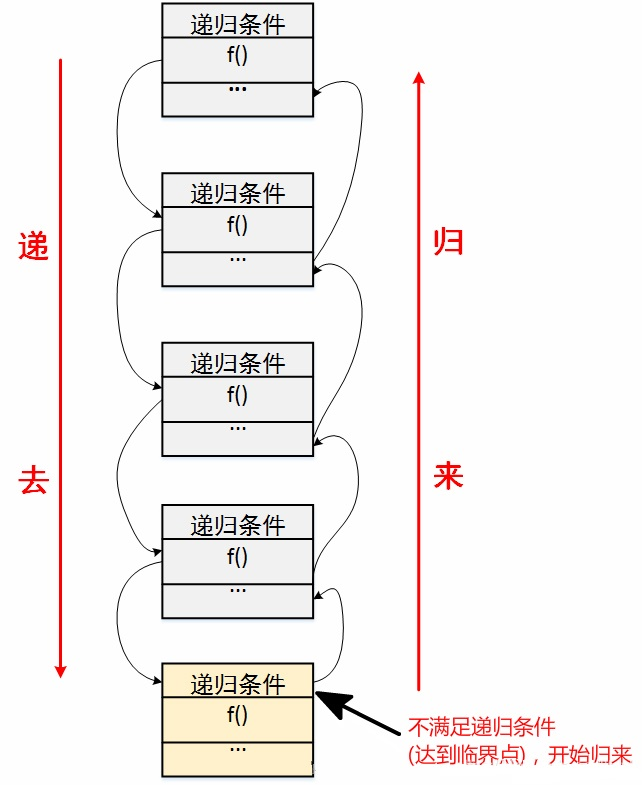
\includegraphics[width=.9\linewidth]{images/recursion.jpg}
          \end{figure} 
        \end{minipage}
\end{frame}

\begin{frame}[fragile]
    \frametitle{斐波纳契数列}
      无穷数列1，1，2，3，5，8，13，21，34，55，… ，被称为Fibonacci数列。
      
      它可以递归地定义为：
      \smallskip

      $f(n) = \begin{cases}
        1 \qquad \qquad \qquad \qquad \quad ~n=1 \qquad \text{边界条件}\\
        1 \qquad \qquad \qquad \qquad \quad ~n=2 \qquad \text{边界条件}\\
        f(n-1) + f(n-2) \qquad n>2  \qquad \text{递归方程}
      \end{cases}$
      \smallskip

\begin{codeblock}{斐波纳契数列}
  def fibonacci(n):
      if n <= 2:
          return 1
      return fibonacci(n - 1) + fibonacci(n - 2)
\end{codeblock}
\end{frame}


\begin{frame}
    \frametitle{斐波纳契数列问题的时间复杂度}
    \begin{figure}[htpb]
      \centering
      
\includegraphics[width=.6\linewidth]{斐波纳契}
    \end{figure}
    存在重叠子问题

    时间复杂度$O(2^n)$ 指数级
\end{frame}


\begin{frame}[fragile]
    \frametitle{使用备忘录进行优化}
\begin{codeblock}{备忘录优化}
memo = {0: 0, 1: 1}
def fib(n):
    if n in memo:
        return memo[n]
    memo[n] = fib(n - 1) + fib(n - 2)
    return memo[n]
\end{codeblock}
备忘录相当于为整个递归遍历树进行了一个剪枝操作。

时间复杂度降为 $O(n)$ ，线性复杂度
\end{frame}


\begin{frame}[t]
    \frametitle{}
    \begin{example}
      一个台阶总共有n级，如果一次可以跳1级，也可以跳2级。总共有多少种跳法？
    \end{example}
    \begin{figure}[htpb]
      \centering
      
\includegraphics[width=.67\linewidth]{跳台阶}
    \end{figure}
\end{frame}


\begin{frame}
    \frametitle{跳台阶问题}
    
      \begin{itemize}
        \item 如果只有1 级台阶，只有一种跳法；
        \item 2级台阶有两种跳法：一种是分两次跳，每次跳1 级；另外一种就是一次跳2 级。
        \item n>2级台阶：
          \begin{itemize}
            \item 第一次只跳1 级，此时跳法数目等于后面剩下的n-1 级台阶的跳法数目，即为f(n-1)；
            \item 第一次跳2 级，此时跳法数目等于后面剩下的n-2 级台阶的跳法数目，即为f(n-2);
            \item 共f(n-1) + f(n-2)种跳法。
          \end{itemize}        
      \end{itemize}
      \[          
      f(n) = \begin{cases}
        1 \qquad \qquad \qquad \qquad \quad ~n=1 \qquad \text{边界条件}\\
        2 \qquad \qquad \qquad \qquad \quad ~n=2 \qquad \text{边界条件}\\
        f(n-1) + f(n-2) \qquad n>2  \qquad \text{递归方程}
      \end{cases}
      \]
\end{frame}

\begin{frame}
    \frametitle{递归和迭代的区别}    
    \begin{center}      
      {\Large \cbf{“To iterate is human, to recurse, divine. — L. Peter Deutsch” }}

      {\Large \cbf{迭代的是人，递归的是神。}}

    \end{center}

    人的常规思维被称为递推（iterate）思维。递推是人类本能的正向思维，而“递归”则有一定的反常识。

    以计算一个整数的阶乘为例，比如5！＝1×2×3×4×5，那么做法是从小到大一个数一个数接连相乘。在生活中，这种做法不仅合情合理，而且浑然天成。
    
    递归算法是怎么计算阶乘的呢？它是倒着来的。比如要算5！，就把它变成5×4！但是4！还不知道呢！但没关系，采用同样的方法，把4！变成4×3！最后到1！时，1！＝1（这就是递归的终止条件）。接下来，就是倒推回所有的结果。

      \begin{center}      
      {\Large \cbf{“人的本质是复读机，不是挖掘机。”}}
    \end{center}

    
\end{frame}

\subsection{贪心算法}

\begin{frame}
    \frametitle{贪心算法}
    贪心算法，是寻找最优解问题的常用方法。这种方法模式一般将求解过程分成若干个步骤，在每个步骤都应用贪心原则，选取当前状态下最好的或最优的选择（局部最有利的选择），并以此希望最后堆叠出的结果也是最好或最优的解。贪心算法的每次决策都以当前情况为基础并根据某个最优原则进行选择，不从整体上考虑其他各种可能的情况。
    \bigskip

    贪心算法只在很少的情况下可以得到真正的最优解。大多数情况下，由于选择策略的“短视”，贪心算法会错过真正的最优解，得不到问题的真正答案。但是贪心算法简单高效，省去了为找最优解可能需要的穷举操作，可以得到与最优解比较接近的近似最优解，通常作为其他算法的辅助算法使用。
\end{frame}

\begin{frame}
    \frametitle{0-1背包问题}
            有一个背包，最多能装下5L的物品，现在有4块蛋糕（蛋糕不能分割），要求在可以装进去的前提下，所装入的物品总价值最高。
\begin{table}[]
  \begin{tabular}{@{}ccccc@{}}
  \toprule
  物品    & 红蛋糕 & 黄蛋糕 & 绿蛋糕 & 白蛋糕 \\ \midrule
  价值(元) & 24  & 10  & 15  & 25  \\
  体积(L) & 3   & 1   & 2   & 4   \\ \bottomrule
  \end{tabular}
  \end{table}       
          \pause
            \begin{minipage}{0.68\linewidth}
              \begin{figure}[htpb]
                \centering
                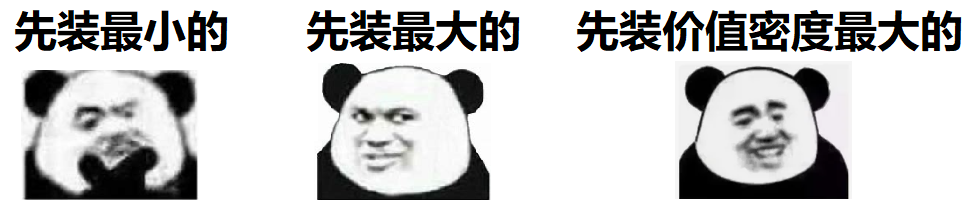
\includegraphics[width=\linewidth]{images/tanxin.png}
              \end{figure}
              \pause
              \vspace{-1em}
              黄+绿=25 \qquad  白+黄=35 \qquad \quad 黄+红=34
              \pause
              \end{minipage}\hfill
              \begin{minipage}{0.28\linewidth}
                  \begin{figure}[htpb]
                    \centering
                    
\includegraphics[width=\linewidth]{images/tanxin2.png}
                  \end{figure}
                  \vspace{-1em}
                  \qquad 红+绿=39
              \end{minipage}
          
\end{frame}

% \begin{frame}
%     \frametitle{贪心算法的基本思想}
%     \begin{enumerate}
%       \item 建立对问题精确描述的数学模型，包括定义最优解的模型；
%       \item 将问题分解为一系列子问题，同时定义子问题的最优解结构；
%       \item 应用贪心原则确定每个子问题的局部最优解，并根据最优解的模型，用子
%       问题的局部最优解堆叠出全局最优解。
%     \end{enumerate}
%     \begin{block}{找零钱}
%       某国发行的货币有25分、10分、5分和1分四种硬币，假如你是售货员，你要找给客户41分钱的硬币，如何安排能使得找给客人的钱正确，但是硬币个数最少。
%       \smallskip
%       \pause

%       定义子问题：从四种币值的硬币中选择一枚，使这个硬币的币值和其他已经选择的硬币的币值总和不超过41分钱。
%       \smallskip

%       子问题的最优解结构：在已经选择的硬币加上当前选择的一枚硬币，当然，选择策略是贪心策略，即在币值总和不超过41的前提下选择币值最大的那种硬币。
%       \smallskip

%       结果：第一次25分的硬币一枚，第二次选择10分的硬币一枚，第三次选择5分的硬币一枚，第四次选择1分的硬币一枚，总共需要4枚硬币。
%     \end{block}
% \end{frame}

% \begin{frame}
%     \frametitle{贪心算法}
%     上面的例子得到的确实是一个最优解，但是很多情况下贪婪法都不能得到最优解。
%     \begin{block}{找零钱2}
%       某国发行的货币有25分、20分、5分和1分四种硬币，假如你是售货员，你要找给客户41分钱的硬币，如何安排能使得找给客人的钱正确，但是硬币个数最少。
%       \smallskip
%       \pause

%       贪心算法结果：1枚25分硬币，三枚5分硬币和一枚1分硬币共5枚硬币。
%       \smallskip

%       实际最优策略：2枚20分的硬币加一枚1分硬币共3枚硬币。
%     \end{block}
% \end{frame}

% \begin{frame}
%     \frametitle{贪心算法}
%     \begin{block}{0-1背包问题}
%       有一个背包，最多能承载重量为$C=150$的物品，现在有7个物品（物品不能分割），编号为1～7，重量分别是$w_i=[35,30,60,50,40,10,25]$，价值分别是$p_i =[10,40,30,50,35,40,30]$，现在从这7个物品中选择一个或多个装入背包，要求在物品总重量不超过$C$的前提下，所装入的物品总价值最高。
%       \smallskip
%     \pause

%       定义子问题：在被背包容量还有$C'$的情况下，选择一个物品装入背包。
%     \smallskip

%     那么如何选择物品呢？对于本题，常见的贪婪策略有三种。
%     \begin{itemize}
%       \item 根据物品价值选择，每次都选价值最高的物品。
      
%       装入背包的物品编号依次是4、2、6、5，此时包中物品总重量是130，总价值是165。
%       \item 根据物品重量选择，每次都选择重量最轻的物品。
      
%       装入背包的物品编号依次是6、7、2、1、5，此时包中物品总重量是140，总价值是155。
%       \item 根据物品价值密度选择，每次选择都选价值密度最高的物品。
      
%       装入背包的物品编号依次是6、2、7、4、1，此时包中物品的总重量是150，总价值是170。
%     \end{itemize}
%     \end{block}         
% \end{frame}

\subsection{动态规划}

\begin{frame}
    \frametitle{动态规划}
    动态规划（dynamic programming）是解决多阶段决策问题常用的最优化理论，该理论由美国数学家Bellman等人在1957年提出，用于研究多阶段决策过程的优化问题。该理论提出后，立即在数学、计算机科学、经济管理和工程技术领域得到了广泛的应用，例如最短路线、库存管理、资源分配、设备更新、排序、装载等问题，用动态规划方法往往比朴素的方法更高效。动态规划方法的原理就是把多阶段决策过程转化为一系列的单阶段决策问题，利用各个阶段之间的递推关系，逐个确定每个阶段的最优化决策，最终堆叠出多阶段决策的最优化决策结果。
\end{frame}


\begin{frame}
    \frametitle{生鲜运输最短路径问题}
      \begin{minipage}{0.48\linewidth}
        生鲜运输注重时效性，运输要求时间尽可能短。

        如图所示，忽略运输其他的影响因素，运输时间最短就是距离最小。图中0表示生鲜农产品运输的起源地，中间可以经过10个地方最后才能到达目的地11，图中的边表示两个地点之间有路，边上的数字表示两个地点的距离，求解单向通行时从源点0到目的地11的最短运输时间，限制条件不走回头路。
    
        \end{minipage}\hfill
        \begin{minipage}{0.48\linewidth}
            \begin{center}
              \begin{tikzpicture}[semithick,node distance=1.5cm,scale=0.8,every node/.style={scale=0.8}]
                \node (0) [circle,minimum width=0.8cm,draw] {0};
                \node (1) [circle,draw,minimum width=0.8cm,right of=0,yshift=2cm] {1};
                \node (2) [circle,draw,minimum width=0.8cm,right of=0,yshift=0.75cm] {2};
                \node (3) [circle,draw,minimum width=0.8cm,right of=0,yshift=-0.75cm] {3};
                \node (4) [circle,draw,minimum width=0.8cm,right of=0,yshift=-2cm] {4};
                \node (5) [circle,draw,minimum width=0.8cm,right of=1,yshift=-0.75cm,xshift=1cm] {5};
                \node (6) [circle,draw,minimum width=0.8cm,right of=1,yshift=-2cm,xshift=1cm] {6};
                \node (7) [circle,draw,minimum width=0.8cm,right of=3,yshift=-0.75cm,xshift=1cm] {7};
                \node (8) [circle,draw,minimum width=0.8cm,right of=5,xshift=1cm] {8};
                \node (9) [circle,draw,minimum width=0.8cm,right of=6,xshift=1cm] {9};
                \node (10) [circle,draw,minimum width=0.8cm,right of=7,xshift=1cm] {10 };
                \node (11)  [circle,draw,minimum width=0.8cm,right of=9] {11};
                \draw [->] (0) -- (1) node [above,midway] {9};
                \draw [->] (0) -- (2) node [above,midway] {7};
                \draw [->] (0) -- (3) node [above,midway] {3};
                \draw [->] (0) -- (4) node [above,midway] {2};
                \draw [->,LightPink2] (1) -- (5) node [above,near end] {4};
                \draw [->,LightPink2] (1) -- (6) node [above,near end] {2};
                \draw [->,LightPink2] (1) -- (7) node [above,near end] {1};
                \draw [->,cyan] (2) -- (5) node [above,midway] {2};
                \draw [->,cyan] (2) -- (6) node [above,midway] {7};
                \draw [->,MediumPurple1] (3) -- (7) node [above,near end] {11};
                \draw [->,SeaGreen2] (4) -- (6) node [above,midway] {11};
                \draw [->,SeaGreen2] (4) -- (7) node [above,midway] {8};
                \draw [->,LightPink2] (5) -- (8) node [above,near end] {6};
                \draw [->,LightPink2] (5) -- (9) node [above,near end] {5};
                \draw [->,cyan] (6) -- (8) node [above,midway] {4};
                \draw [->,cyan] (6) -- (9) node [above,midway] {3};
                \draw [->,MediumPurple1] (7) -- (9) node [above,midway] {5};
                \draw [->,MediumPurple1] (7) -- (10) node [above,midway] {6};
                \draw [->] (8) -- (11) node [above,midway] {4};
                \draw [->] (9) -- (11) node [above,midway] {2};
                \draw [->] (10) -- (11) node [above,midway] {5};
            \end{tikzpicture}
            \end{center}
        \end{minipage}
\end{frame}

\begin{frame}
    \frametitle{动态规划特点}
    每种方法都有自身的局限性，动态规划法也不是万能的。动态规划适合求解多阶段（状态转换）决策问题的最优解，也可用于含有线性或非线性递推关系的最优解问题，但是这些问题都必须满足最优化原理和子问题的“无后向性”。
    \begin{itemize}
      \item {\cbf{最优化原理}}
      
      不管之前决策是否是最优决策，都必须保证从现在开始的决策是在之前决策基础上的最优决策。
      \item {\cbf{无后向性（无后效性）}}
      
      每个阶段的决策仅受之前决策的影响，但是不影响之后各阶段的决策。
    \end{itemize}
\end{frame}

\begin{frame}
    \frametitle{动态规划基本思想}
    和分治法一样，动态规划解决复杂问题的思路也是对问题进行分解，通过求解小规模的子问题再反推出原问题的结果。但是动态规划分解子问题不是简单地按照“大事化小”的方式进行的，而是沿着决策的阶段划分子问题，决策的阶段可以随时间划分，也可以随着问题的演化状态划分。分治法要求子问题是互相独立的，以便分别求解并最终合并出原始问题的解，但是动态规划法的子问题不是互相独立的，子问题之间通常有包含关系，甚至两个子问题可以包含相同的子子问题。除此之外，动态规划法的子问题还要满足“无后向性”要求。
\end{frame}

\begin{frame}
    \frametitle{动态规划求解步骤}
    \begin{enumerate}
      \small
      \item {\cbf{划分阶段}}
      
      划分阶段没有固定的方法，根据问题的结构，可以按照时间顺序划分阶段，也可以按照问题的演化状态划分阶段。阶段划分以后，对问题的求解就变成对各个阶段分别进行最优化决策，问题的解就变成按照阶段顺序依次选择的一个决策序列。
      \item {\cbf{确定状态}}
      
      对于每个阶段来说，对起始状态施加决策，使得状态发生改变，得到决策的结果状态。初始状态经过每一个阶段的决策（状态改变）之后，最终得到的状态就是问题的解。
      \item {\cbf{确定决策并写出状态转移方程}}
    
      决策就是能使状态发生转变的选择动作，如果选择动作有多个，则决策就是取其中能使得阶段结果最优的那一个。状态转换方程是描述状态转换关系的一系列等式，也就是从n-1 阶段到n 阶段演化的规律。
      \item {\cbf{确定边界条件}}
    
      给出的状态转移方程是一个递推式，需要一个递推的终止条件或边界条件。
    \end{enumerate}
\end{frame}

\begin{frame}
  \frametitle{动态规划求解步骤}
  \begin{center}
    \only<1>{
    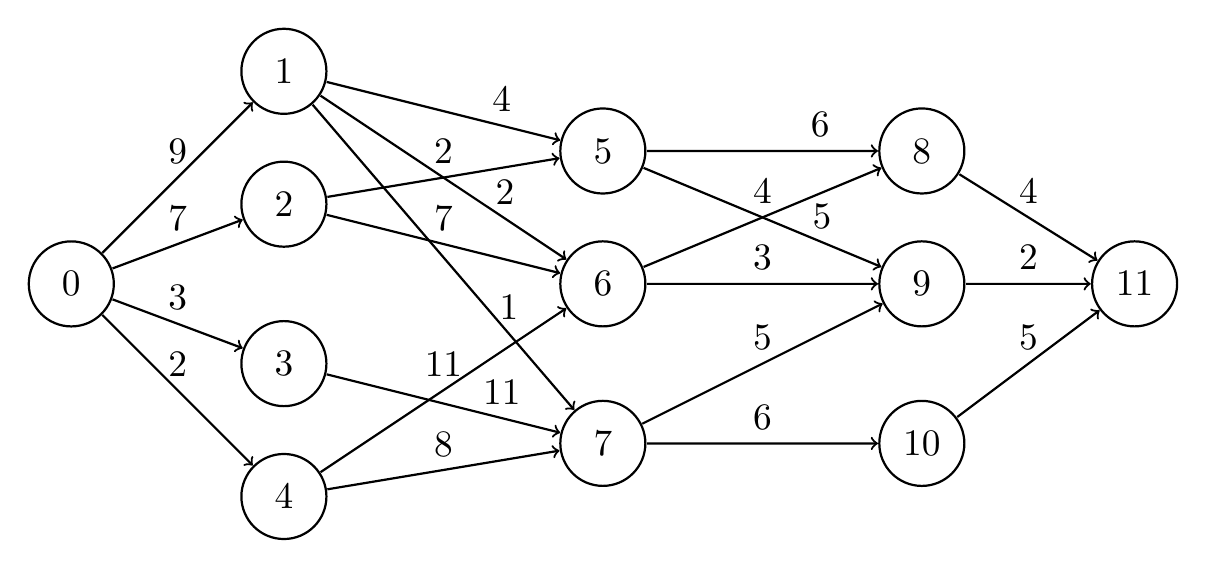
\begin{tikzpicture}[thick,node distance=2cm,scale=1.35,every node/.style={scale=1.35}]
      \node (0) [circle,minimum width=0.8cm,draw] {0};
      \node (1) [circle,draw,minimum width=0.8cm,right of=0,yshift=2cm] {1};
      \node (2) [circle,draw,minimum width=0.8cm,right of=0,yshift=0.75cm] {2};
      \node (3) [circle,draw,minimum width=0.8cm,right of=0,yshift=-0.75cm] {3};
      \node (4) [circle,draw,minimum width=0.8cm,right of=0,yshift=-2cm] {4};
      \node (5) [circle,draw,minimum width=0.8cm,right of=1,yshift=-0.75cm,xshift=1cm] {5};
      \node (6) [circle,draw,minimum width=0.8cm,right of=1,yshift=-2cm,xshift=1cm] {6};
      \node (7) [circle,draw,minimum width=0.8cm,right of=3,yshift=-0.75cm,xshift=1cm] {7};
      \node (8) [circle,draw,minimum width=0.8cm,right of=5,xshift=1cm] {8};
      \node (9) [circle,draw,minimum width=0.8cm,right of=6,xshift=1cm] {9};
      \node (10) [circle,draw,minimum width=0.8cm,right of=7,xshift=1cm] {10 };
      \node (11)  [circle,draw,minimum width=0.8cm,right of=9] {11};
      \draw [->] (0) -- (1) node [above,midway] {9};
      \draw [->] (0) -- (2) node [above,midway] {7};
      \draw [->] (0) -- (3) node [above,midway] {3};
      \draw [->] (0) -- (4) node [above,midway] {2};
      \draw [->] (1) -- (5) node [above,near end] {4};
      \draw [->] (1) -- (6) node [above,near end] {2};
      \draw [->] (1) -- (7) node [above,near end] {1};
      \draw [->] (2) -- (5) node [above,midway] {2};
      \draw [->] (2) -- (6) node [above,midway] {7};
      \draw [->] (3) -- (7) node [above,near end] {11};
      \draw [->] (4) -- (6) node [above,midway] {11};
      \draw [->] (4) -- (7) node [above,midway] {8};
      \draw [->] (5) -- (8) node [above,near end] {6};
      \draw [->] (5) -- (9) node [above,near end] {5};
      \draw [->,] (6) -- (8) node [above,midway] {4};
      \draw [->] (6) -- (9) node [above,midway] {3};
      \draw [->] (7) -- (9) node [above,midway] {5};
      \draw [->] (7) -- (10) node [above,midway] {6};
      \draw [->] (8) -- (11) node [above,midway] {4};
      \draw [->] (9) -- (11) node [above,midway] {2};
      \draw [->] (10) -- (11) node [above,midway] {5};
  \end{tikzpicture}
  }
  \only<2>{
    \begin{tikzpicture}[thick,node distance=2cm,scale=1.35,every node/.style={scale=1.35}]
      \node (0) [circle,minimum width=0.8cm,draw] {0};
      \node (1) [circle,draw,minimum width=0.8cm,right of=0,yshift=2cm] {1};
      \node (2) [circle,draw,minimum width=0.8cm,right of=0,yshift=0.75cm] {2};
      \node (3) [circle,draw,minimum width=0.8cm,right of=0,yshift=-0.75cm] {3};
      \node (4) [circle,draw,minimum width=0.8cm,right of=0,yshift=-2cm] {4};
      \node (5) [circle,draw,minimum width=0.8cm,right of=1,yshift=-0.75cm,xshift=1cm] {5};
      \node (6) [circle,draw,minimum width=0.8cm,right of=1,yshift=-2cm,xshift=1cm] {6};
      \node (7) [circle,draw,minimum width=0.8cm,right of=3,yshift=-0.75cm,xshift=1cm] {7};
      \node (8) [circle,draw,minimum width=0.8cm,right of=5,xshift=1cm] {8};
      \node (9) [circle,draw,minimum width=0.8cm,right of=6,xshift=1cm] {9};
      \node (10) [circle,draw,minimum width=0.8cm,right of=7,xshift=1cm] {10 };
      \node (11)  [circle,draw,minimum width=0.8cm,right of=9] {11};
      \draw [->] (0) -- (1) node [above,midway] {9};
      \draw [->] (0) -- (2) node [above,midway] {7};
      \draw [->] (0) -- (3) node [above,midway] {3};
      \draw [->] (0) -- (4) node [above,midway] {2};
      \draw [->] (1) -- (5) node [above,near end] {4};
      \draw [->] (1) -- (6) node [above,near end] {2};
      \draw [->] (1) -- (7) node [above,near end] {1};
      \draw [->] (2) -- (5) node [above,midway] {2};
      \draw [->] (2) -- (6) node [above,midway] {7};
      \draw [->] (3) -- (7) node [above,near end] {11};
      \draw [->] (4) -- (6) node [above,midway] {11};
      \draw [->] (4) -- (7) node [above,midway] {8};
      \draw [->] (5) -- (8) node [above,near end] {6};
      \draw [->] (5) -- (9) node [above,near end] {5};
      \draw [->,] (6) -- (8) node [above,midway] {4};
      \draw [->] (6) -- (9) node [above,midway] {3};
      \draw [->] (7) -- (9) node [above,midway] {5};
      \draw [->] (7) -- (10) node [above,midway] {6};
      \draw [->] (8) -- (11) node [above,midway] {4};
      \draw [->] (9) -- (11) node [above,midway] {2};
      \draw [->] (10) -- (11) node [above,midway] {5};
      \draw [thin,dashed,DeepSkyBlue2] (0,-2.5) -- (0,2.25);
    \draw [thin,dashed,DeepSkyBlue2,shift={(2,0)}] (0,-2.5) -- (0,2.25);
    \draw [thin,dashed,DeepSkyBlue2,shift={(5,0)}] (0,-2.5) -- (0,2.25);
    \draw [thin,dashed,DeepSkyBlue2,shift={(8,0)}] (0,-2.5) -- (0,2.25);
    \draw [thin,dashed,DeepSkyBlue2,shift={(10,0)}] (0,-2.5) -- (0,2.25);
    \node at (1,-2.5) {第4阶段};
    \node at (3.5,-2.5) {第3阶段};
    \node at (6.5,-2.5) {第2阶段};
    \node at (9,-2.5) {第1阶段};
  \end{tikzpicture}
  }
  \only<3>{
    \begin{tikzpicture}[thick,node distance=2cm,scale=1.35,every node/.style={scale=1.35}]
      \node (0) [circle,minimum width=0.8cm,draw] {0};
      \node (1) [circle,draw,minimum width=0.8cm,right of=0,yshift=2cm] {1};
      \node (2) [circle,draw,minimum width=0.8cm,right of=0,yshift=0.75cm] {2};
      \node (3) [circle,draw,minimum width=0.8cm,right of=0,yshift=-0.75cm] {3};
      \node (4) [circle,draw,minimum width=0.8cm,right of=0,yshift=-2cm] {4};
      \node (5) [circle,draw,minimum width=0.8cm,right of=1,yshift=-0.75cm,xshift=1cm] {5};
      \node (6) [circle,draw,minimum width=0.8cm,right of=1,yshift=-2cm,xshift=1cm] {6};
      \node (7) [circle,draw,minimum width=0.8cm,right of=3,yshift=-0.75cm,xshift=1cm] {7};
      \node (8) [circle,draw,minimum width=0.8cm,right of=5,xshift=1cm] {8};
      \node (9) [circle,draw,minimum width=0.8cm,right of=6,xshift=1cm] {9};
      \node (10) [circle,draw,minimum width=0.8cm,right of=7,xshift=1cm] {10 };
      \node (11)  [circle,draw,minimum width=0.8cm,right of=9] {11};
      \draw [->] (0) -- (1) node [above,midway] {9};
      \draw [->] (0) -- (2) node [above,midway] {7};
      \draw [->] (0) -- (3) node [above,midway] {3};
      \draw [->] (0) -- (4) node [above,midway] {2};
      \draw [->] (1) -- (5) node [above,near end] {4};
      \draw [->] (1) -- (6) node [above,near end] {2};
      \draw [->] (1) -- (7) node [above,near end] {1};
      \draw [->] (2) -- (5) node [above,midway] {2};
      \draw [->] (2) -- (6) node [above,midway] {7};
      \draw [->] (3) -- (7) node [above,near end] {11};
      \draw [->] (4) -- (6) node [above,midway] {11};
      \draw [->] (4) -- (7) node [above,midway] {8};
      \draw [->] (5) -- (8) node [above,near end] {6};
      \draw [->] (5) -- (9) node [above,near end] {5};
      \draw [->,] (6) -- (8) node [above,midway] {4};
      \draw [->] (6) -- (9) node [above,midway] {3};
      \draw [->] (7) -- (9) node [above,midway] {5};
      \draw [->] (7) -- (10) node [above,midway] {6};
      \draw [->,cyan] (8) -- (11) node [above,midway] {4};
      \draw [->,MediumPurple1] (9) -- (11) node [above,midway] {2};
      \draw [->,LightPink2] (10) -- (11) node [above,midway] {5};
      \draw [thin,dashed,DeepSkyBlue2] (0,-2.5) -- (0,2.25);
    \draw [thin,dashed,DeepSkyBlue2,shift={(2,0)}] (0,-2.5) -- (0,2.25);
    \draw [thin,dashed,DeepSkyBlue2,shift={(5,0)}] (0,-2.5) -- (0,2.25);
    \draw [thin,dashed,DeepSkyBlue2,shift={(8,0)}] (0,-2.5) -- (0,2.25);
    \draw [thin,dashed,DeepSkyBlue2,shift={(10,0)}] (0,-2.5) -- (0,2.25);
    \node at (1,-2.5) {第4阶段};
    \node at (3.5,-2.5) {第3阶段};
    \node at (6.5,-2.5) {第2阶段};
    \node at (9,-2.5) {第1阶段};
  \end{tikzpicture}
  }
  \only<4>{
    \begin{tikzpicture}[thick,node distance=2cm,scale=1.35,every node/.style={scale=1.35}]
      \node (0) [circle,minimum width=0.8cm,draw] {0};
      \node (1) [circle,draw,minimum width=0.8cm,right of=0,yshift=2cm] {1};
      \node (2) [circle,draw,minimum width=0.8cm,right of=0,yshift=0.75cm] {2};
      \node (3) [circle,draw,minimum width=0.8cm,right of=0,yshift=-0.75cm] {3};
      \node (4) [circle,draw,minimum width=0.8cm,right of=0,yshift=-2cm] {4};
      \node (5) [circle,draw,minimum width=0.8cm,right of=1,yshift=-0.75cm,xshift=1cm] {5};
      \node (6) [circle,draw,minimum width=0.8cm,right of=1,yshift=-2cm,xshift=1cm] {6};
      \node (7) [circle,draw,minimum width=0.8cm,right of=3,yshift=-0.75cm,xshift=1cm] {7};
      \node (8) [circle,draw,minimum width=0.8cm,right of=5,xshift=1cm] {8};
      \node (9) [circle,draw,minimum width=0.8cm,right of=6,xshift=1cm] {9};
      \node (10) [circle,draw,minimum width=0.8cm,right of=7,xshift=1cm] {10 };
      \node (11)  [circle,draw,minimum width=0.8cm,right of=9] {11};
      \draw [->] (0) -- (1) node [above,midway] {9};
      \draw [->] (0) -- (2) node [above,midway] {7};
      \draw [->] (0) -- (3) node [above,midway] {3};
      \draw [->] (0) -- (4) node [above,midway] {2};
      \draw [->] (1) -- (5) node [above,near end] {4};
      \draw [->] (1) -- (6) node [above,near end] {2};
      \draw [->] (1) -- (7) node [above,near end] {1};
      \draw [->] (2) -- (5) node [above,midway] {2};
      \draw [->] (2) -- (6) node [above,midway] {7};
      \draw [->] (3) -- (7) node [above,near end] {11};
      \draw [->] (4) -- (6) node [above,midway] {11};
      \draw [->] (4) -- (7) node [above,midway] {8};
      \draw [->] (5) -- (8) node [above,near end] {6};
      \draw [->,cyan] (5) -- (9) node [above,near end] {5(7)};
      \draw [->] (6) -- (8) node [above,midway] {4};
      \draw [->,MediumPurple1] (6) -- (9) node [above,midway] {3(5)};
      \draw [->,LightPink2] (7) -- (9) node [above,midway] {5(7)};
      \draw [->] (7) -- (10) node [above,midway] {6};
      \draw [->] (8) -- (11) node [above,midway] {4};
      \draw [->,MediumPurple1] (9) -- (11);
      \draw [->] (10) -- (11) node [above,midway] {5};
      \draw [thin,dashed,DeepSkyBlue2] (0,-2.5) -- (0,2.25);
    \draw [thin,dashed,DeepSkyBlue2,shift={(2,0)}] (0,-2.5) -- (0,2.25);
    \draw [thin,dashed,DeepSkyBlue2,shift={(5,0)}] (0,-2.5) -- (0,2.25);
    \draw [thin,dashed,DeepSkyBlue2,shift={(8,0)}] (0,-2.5) -- (0,2.25);
    \draw [thin,dashed,DeepSkyBlue2,shift={(10,0)}] (0,-2.5) -- (0,2.25);
    \node at (1,-2.5) {第4阶段};
    \node at (3.5,-2.5) {第3阶段};
    \node at (6.5,-2.5) {第2阶段};
    \node at (9,-2.5) {第1阶段};
  \end{tikzpicture}
  }
  \only<5>{
    \begin{tikzpicture}[thick,node distance=2cm,scale=1.35,every node/.style={scale=1.35}]
      \node (0) [circle,minimum width=0.8cm,draw] {0};
      \node (1) [circle,draw,minimum width=0.8cm,right of=0,yshift=2cm] {1};
      \node (2) [circle,draw,minimum width=0.8cm,right of=0,yshift=0.75cm] {2};
      \node (3) [circle,draw,minimum width=0.8cm,right of=0,yshift=-0.75cm] {3};
      \node (4) [circle,draw,minimum width=0.8cm,right of=0,yshift=-2cm] {4};
      \node (5) [circle,draw,minimum width=0.8cm,right of=1,yshift=-0.75cm,xshift=1cm] {5};
      \node (6) [circle,draw,minimum width=0.8cm,right of=1,yshift=-2cm,xshift=1cm] {6};
      \node (7) [circle,draw,minimum width=0.8cm,right of=3,yshift=-0.75cm,xshift=1cm] {7};
      \node (8) [circle,draw,minimum width=0.8cm,right of=5,xshift=1cm] {8};
      \node (9) [circle,draw,minimum width=0.8cm,right of=6,xshift=1cm] {9};
      \node (10) [circle,draw,minimum width=0.8cm,right of=7,xshift=1cm] {10 };
      \node (11)  [circle,draw,minimum width=0.8cm,right of=9] {11};
      \draw [->] (0) -- (1) node [above,midway] {9};
      \draw [->] (0) -- (2) node [above,midway] {7};
      \draw [->] (0) -- (3) node [above,midway] {3};
      \draw [->] (0) -- (4) node [above,midway] {2};
      \draw [->] (1) -- (5) node [above,near end] {4};
      \draw [->,MediumPurple1] (1) -- (6) node [above,near end] {2(7)};
      \draw [->] (1) -- (7) node [above,near end] {1};
      \draw [->,cyan] (2) -- (5) node [above,midway] {2(9)};
      \draw [->] (2) -- (6) node [above,midway] {7};
      \draw [->,LightPink2] (3) -- (7) node [above,near end] {11(18)};
      \draw [->] (4) -- (6) node [above,midway] {11};
      \draw [->,Chartreuse3] (4) -- (7) node [above,midway] {8(15)};
      \draw [->] (5) -- (8) node [above,near end] {6};
      \draw [->,cyan] (5) -- (9) node [above,near end] {5};
      \draw [->] (6) -- (8) node [above,midway] {4};
      \draw [->,MediumPurple1] (6) -- (9) node [above,midway] {3};
      \draw [->,LightPink2] (7) -- (9) node [above,midway] {5};
      \draw [->] (7) -- (10) node [above,midway] {6};
      \draw [->] (8) -- (11) node [above,midway] {4};
      \draw [->,MediumPurple1] (9) -- (11);
      \draw [->] (10) -- (11) node [above,midway] {5};
      \draw [thin,dashed,DeepSkyBlue2] (0,-2.5) -- (0,2.25);
    \draw [thin,dashed,DeepSkyBlue2,shift={(2,0)}] (0,-2.5) -- (0,2.25);
    \draw [thin,dashed,DeepSkyBlue2,shift={(5,0)}] (0,-2.5) -- (0,2.25);
    \draw [thin,dashed,DeepSkyBlue2,shift={(8,0)}] (0,-2.5) -- (0,2.25);
    \draw [thin,dashed,DeepSkyBlue2,shift={(10,0)}] (0,-2.5) -- (0,2.25);
    \node at (1,-2.5) {第4阶段};
    \node at (3.5,-2.5) {第3阶段};
    \node at (6.5,-2.5) {第2阶段};
    \node at (9,-2.5) {第1阶段};
  \end{tikzpicture}
  }
  \only<6>{
    \begin{tikzpicture}[thick,node distance=2cm,scale=1.35,every node/.style={scale=1.35}]
      \node (0) [circle,minimum width=0.8cm,draw] {0};
      \node (1) [circle,draw,minimum width=0.8cm,right of=0,yshift=2cm] {1};
      \node (2) [circle,draw,minimum width=0.8cm,right of=0,yshift=0.75cm] {2};
      \node (3) [circle,draw,minimum width=0.8cm,right of=0,yshift=-0.75cm] {3};
      \node (4) [circle,draw,minimum width=0.8cm,right of=0,yshift=-2cm] {4};
      \node (5) [circle,draw,minimum width=0.8cm,right of=1,yshift=-0.75cm,xshift=1cm] {5};
      \node (6) [circle,draw,minimum width=0.8cm,right of=1,yshift=-2cm,xshift=1cm] {6};
      \node (7) [circle,draw,minimum width=0.8cm,right of=3,yshift=-0.75cm,xshift=1cm] {7};
      \node (8) [circle,draw,minimum width=0.8cm,right of=5,xshift=1cm] {8};
      \node (9) [circle,draw,minimum width=0.8cm,right of=6,xshift=1cm] {9};
      \node (10) [circle,draw,minimum width=0.8cm,right of=7,xshift=1cm] {10 };
      \node (11)  [circle,draw,minimum width=0.8cm,right of=9] {11};
      \draw [->,MediumPurple1] (0) -- (1) node [above,midway] {9(16)};
      \draw [->,cyan] (0) -- (2) node [above,midway] {7(16)};
      \draw [->] (0) -- (3) node [above,midway] {3};
      \draw [->] (0) -- (4) node [above,midway] {2};
      \draw [->] (1) -- (5) node [above,near end] {4};
      \draw [->,MediumPurple1] (1) -- (6) node [above,near end] {2};
      \draw [->] (1) -- (7) node [above,near end] {1};
      \draw [->,cyan] (2) -- (5) node [above,midway] {2};
      \draw [->] (2) -- (6) node [above,midway] {7};
      \draw [->] (3) -- (7) node [above,near end] {11};
      \draw [->] (4) -- (6) node [above,midway] {11};
      \draw [->] (4) -- (7) node [above,midway] {8};
      \draw [->] (5) -- (8) node [above,near end] {6};
      \draw [->,cyan] (5) -- (9) node [above,near end] {5};
      \draw [->] (6) -- (8) node [above,midway] {4};
      \draw [->,MediumPurple1] (6) -- (9) node [above,midway] {3};
      \draw [->] (7) -- (9) node [above,midway] {5};
      \draw [->] (7) -- (10) node [above,midway] {6};
      \draw [->] (8) -- (11) node [above,midway] {4};
      \draw [->,MediumPurple1] (9) -- (11);
      \draw [->] (10) -- (11) node [above,midway] {5};
      \draw [thin,dashed,DeepSkyBlue2] (0,-2.5) -- (0,2.25);
    \draw [thin,dashed,DeepSkyBlue2,shift={(2,0)}] (0,-2.5) -- (0,2.25);
    \draw [thin,dashed,DeepSkyBlue2,shift={(5,0)}] (0,-2.5) -- (0,2.25);
    \draw [thin,dashed,DeepSkyBlue2,shift={(8,0)}] (0,-2.5) -- (0,2.25);
    \draw [thin,dashed,DeepSkyBlue2,shift={(10,0)}] (0,-2.5) -- (0,2.25);
    \node at (1,-2.5) {第4阶段};
    \node at (3.5,-2.5) {第3阶段};
    \node at (6.5,-2.5) {第2阶段};
    \node at (9,-2.5) {第1阶段};
  \end{tikzpicture}
  }
  \end{center}
\end{frame}


\begin{frame}[t]
    \frametitle{数塔问题}
    \begin{example}
      有形如图所示的一个数塔，从顶部出发，在每一结点可以选择向左走或是向右走，一直走到底层，要求找出一条路径，使路径上的数值和最大。
      \begin{figure}[htpb]
        \centering
        
\includegraphics[width=.45\linewidth]{数塔}
      \end{figure}
    \end{example}
\end{frame}


\begin{frame}[fragile]
    \frametitle{}
    \begin{codeblock}{}
n = 5
y = [[9], [12, 15], [10, 6, 8], [2, 18, 9, 5], [19, 7, 10, 4, 16]]
for a in range(n - 2, -1, -1):
    for b in range(a + 1):
        y[a][b] = max((y[a][b] + y[a + 1][b]), (y[a][b] + y[a + 1][b + 1])) # 父子相加取大者
        print((a, b), '=', (y[a][b]), end='-------')
    print()
num1 = y[0][0]
print('最大值为:%d' % (num1))
print('经过的数字为:', end='')
m = 0
for k in range(1, n):
    m = y[k].index(max(y[k][m], y[k][m + 1]))
    num2 = y[k][m]
    print(num1 - num2, end='->')
    num1 = num2
    if k == n - 1:
        print(num1)
    \end{codeblock}
    \vspace{-3pt}
\end{frame}


\begin{frame}[t]
    \frametitle{0-1背包问题}
    \begin{example}
      有一个背包，最多能装下5L的物品，现在有4块蛋糕（蛋糕不能分割），要求在可以装进去的前提下，所装入的物品总价值最高。
\begin{table}[]
  \begin{tabular}{@{}ccccc@{}}
  \toprule
  物品    & 红蛋糕 & 黄蛋糕 & 绿蛋糕 & 白蛋糕 \\ \midrule
  价值(元) & 24  & 10  & 15  & 25  \\
  体积(L) & 3   & 1   & 2   & 4   \\ \bottomrule
  \end{tabular}
  \end{table}       
    \end{example}
\end{frame}


\begin{frame}
    \frametitle{0-1背包问题}
    \begin{enumerate}
          \item 如果第 i 件宝物太重，加不到背包中，那么前 i 件宝物价值等于前 i-1 件宝物价值，即 m(i, W) = m(i-1, W)；
          \item 如果第 i 件宝物可以加入到背包中，那么前 i 件宝物价值等于前 i-1 件宝物价值加上第 i 件宝物价值Wi，即 m(i, W) = m(i-1, W-Wi)+vi。
    \end{enumerate}
    因此，m(i, W) 应该是m(i-1, W) 和m(i-1, W-Wi)+vi 两者最大值，即m(i, W) = max{m(i-1, W), m(i-1, W-Wi)+vi}
    \begin{figure}[htpb]
      \centering
      
\includegraphics[width=.9\linewidth]{背包动态规划}
    \end{figure}
\end{frame}


\begin{frame}
    \frametitle{动态规划表格}
    \begin{center}
        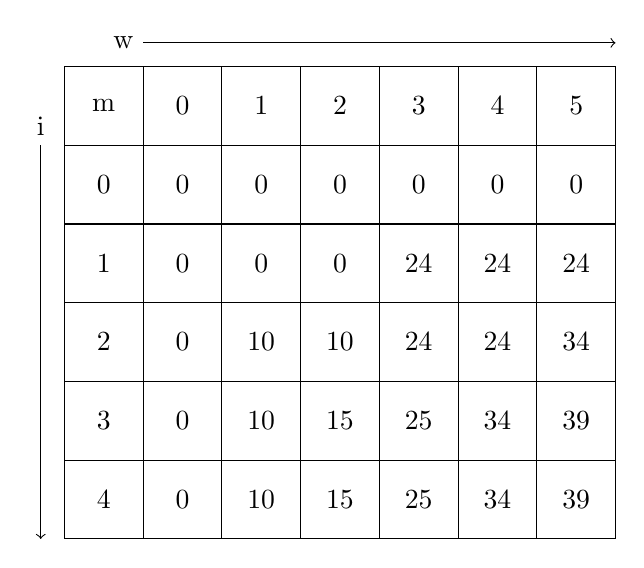
\begin{tikzpicture}
            \foreach [count = \i] \x in {m,0,1,2,3,4,5}
            \draw [shift={(\i,1)}] (0,0) rectangle (1,1) node [midway] {\x};
            \foreach [count = \i] \x in {0,0,0,0,0,0,0}
            \draw [shift={(\i,0)}] (0,0) rectangle (1,1) node [midway] {\x};
            \foreach [count = \i] \x in {1,0,0,0,24,24,24}
            \draw [shift={(\i,-1)}] (0,0) rectangle (1,1) node [midway] {\x};
            \foreach [count = \i] \x in {2,0,10,10,24,24,34}
            \draw [shift={(\i,-2)}] (0,0) rectangle (1,1) node [midway] {\x};
            \foreach [count = \i] \x in {3,0,10,15,25,34,39}
            \draw [shift={(\i,-3)}] (0,0) rectangle (1,1) node [midway] {\x};
            \foreach [count = \i] \x in {4,0,10,15,25,34,39}
            \draw [shift={(\i,-4)}] (0,0) rectangle (1,1) node [midway] {\x};
            \draw[->] (2,2.3) node [left] {w} -- (8,2.3);
            \draw[->] (0.7,1) node [above] {i} -- (0.7,-4);
        \end{tikzpicture}
    \end{center}
\end{frame}


\begin{frame}[fragile]
    \frametitle{}
    \begin{codeblock}{装载宝物}
goods = [None, {'w': 3,'v': 24}, {'w': 1,'v': 10}, {'w': 2,'v': 15}, {'w': 4,'v': 25}]
max_w = 5 # 设置背包最大承重
# 初始化二维表格m[(i, w)]，将表格中所有价值均初始化为0
m = {(i, w): 0 for i in range(len(goods)) for w in range(max_w + 1)}
for i in range(1, len(goods)):
    for w in range(1, max_w + 1):
        if goods[i]['w'] > w:
            # 装不下第i个宝物，即不装第i个宝物
            m[(i, w)] = m[(i - 1, w)]
        else:
            # 装得下第i个宝物时，在不装第i个宝物与装第i个宝物这两种情况下，取最大价值
            m[(i, w)] = max(m[(i - 1, w)], m[(i - 1, w - goods[i]['w'])] + goods[i]['v'])
print(m[(len(goods) - 1, max_w)]) # 输出结果
    \end{codeblock}
\end{frame}





\subsection{回溯法}


\begin{frame}
    \frametitle{回溯法}
    \begin{minipage}{0.48\linewidth}
      「回溯算法」是一种通过穷举来解决问题的方法，它的核心思想是从一个初始状态出发，暴力搜索所有可能的解决方案，当遇到正确的解则将其记录，直到找到解或者尝试了所有可能的选择都无法找到解为止。
      
      当算法在搜索过程中遇到某个状态无法继续前进或无法得到满足条件的解时，它会撤销上一步的选择，退回到之前的状态，并尝试其他可能的选择。
    \end{minipage}\hfill
    \begin{minipage}{0.48\linewidth}
      \begin{figure}[htpb]
        \centering
        
\includegraphics[width=\linewidth]{迷宫}
      \end{figure}
    \end{minipage}
    
\end{frame}


\begin{frame}
    \frametitle{问题解空间}
    应用回溯法求解问题时，首先应明确定义问题的解空间，该解空间应至少包含问题的一个最优解。在定义了问题的解空间后，还需要将解空间有效地组织起来，使得回溯法能方便地搜索整个解空间，通常将解空间组织成子集树和排列树的形式。
    \begin{figure}[htpb]
        \centering
        \setcounter{subfigure}{0}
        \subfloat[子集树]{
\includegraphics[height=4cm]{子集树}}\quad
        \subfloat[排列树]{
\includegraphics[height=4cm]{排列树}}
    \end{figure}
\end{frame}


\begin{frame}
    \frametitle{0-1背包问题}
    给定一背包的容量$C$，和$N$个物品的重量$w_i$价值$v_i$，求在背包容量允许的条件下能装入的最大价值。设$N=3, W=(16,15,15), P=(45,25,25), C=30$
  \begin{figure}[htpb]
    \centering
    
\includegraphics[width=.67\linewidth]{01背包}
  \end{figure}
\end{frame}


\begin{frame}
    \frametitle{旅行商问题}
    某售货员要到若干城市去推销商品，已知各城市之间的路程，他要选定一条从驻地出发，经过每个城市一遍，最后回到驻地的路线，使总的路程最短。
    \begin{figure}[htpb]
      \centering
      
\includegraphics[width=.9\linewidth]{旅行商}
    \end{figure}
\end{frame}











\subsection{分支限界法}


\begin{frame}[t]
    \frametitle{分支限界法}
    \begin{example}
      假定有 N=4 件商品 ， 分别用 A 、 B 、 C 、 D 表示 。 每件商品的重量分别为
      3kg 、 2kg 、 5kg 和 4kg ， 对应的价值分别为 66 元 、 40 元 、 95 元和 40 元 。
      现有一个背包 ， 可以容纳的总重量为 9kg ， 问 ： 如何挑选商品 ， 使得背包里
      商品的总价值最大 ？
    \end{example}
\end{frame}


\begin{frame}
    \frametitle{}
    \begin{center}
      \only<1>{
      
\begin{tikzpicture}[scale=1.45]
        \Tree
    [.O
    [.$A$ 
    [.$B$ [.$C$ [.$D$ ] [.$\bar D$ ] ] [.$\bar C$ [.$D$ ] [.$\bar D$ ] ] ] 
    [.$\bar B$ [.$C$ [.$D$ ] [.$\bar D$ ] ] [.$\bar C$ [.$D$ ] [.$\bar D$ ] ] ] ]
    [.$\bar A$ 
    [.$B$ [.$C$ [.$D$ ] [.$\bar D$ ] ] [.$\bar C$ [.$D$ ] [.$\bar D$ ] ] ] 
    [.$\bar B$ [.$C$ [.$D$ ] [.$\bar D$ ] ] [.$\bar C$ [.$D$ ] [.$\bar D$ ] ] ] ] 
    ]
    \end{tikzpicture}
    }
    \only<2>{
      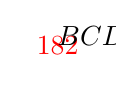
\begin{tikzpicture}[scale=1.45]
        \Tree
    [.O
    [.\node[red]{182}; 
    [.$B$ [.$C$ [.$D$ ] [.$\bar D$ ] ] [.$\bar C$ [.$D$ ] [.$\bar D$ ] ] ] 
    [.$\bar B$ [.$C$ [.$D$ ] [.$\bar D$ ] ] [.$\bar C$ [.$D$ ] [.$\bar D$ ] ] ] ]
    [.\node[red]{155}; 
    [.$B$ [.$C$ [.$D$ ] [.$\bar D$ ] ] [.$\bar C$ [.$D$ ] [.$\bar D$ ] ] ] 
    [.$\bar B$ [.$C$ [.$D$ ] [.$\bar D$ ] ] [.$\bar C$ [.$D$ ] [.$\bar D$ ] ] ] ] 
    ]
    \end{tikzpicture}
    }
    \only<3>{
      
\begin{tikzpicture}[scale=1.45]
        \Tree
    [.O
    [.$A$ 
    [.\node[red]{182};  [.$C$ [.$D$ ] [.$\bar D$ ] ] [.$\bar C$ [.$D$ ] [.$\bar D$ ] ] ] 
    [.\node[red]{171};  [.$C$ [.$D$ ] [.$\bar D$ ] ] [.$\bar C$ [.$D$ ] [.$\bar D$ ] ] ] ]
    [.\node[red]{155}; 
    [.$B$ [.$C$ [.$D$ ] [.$\bar D$ ] ] [.$\bar C$ [.$D$ ] [.$\bar D$ ] ] ] 
    [.$\bar B$ [.$C$ [.$D$ ] [.$\bar D$ ] ] [.$\bar C$ [.$D$ ] [.$\bar D$ ] ] ] ] 
    ]
    \end{tikzpicture}
    }
    \only<4>{
      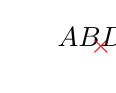
\begin{tikzpicture}[scale=1.45]
        \Tree
    [.O
    [.$A$ 
    [.$B$  [.\node[red]{$\times$}; [.$D$ ] [.$\bar D$ ] ] [.\node[red]{146}; [.$D$ ] [.$\bar D$ ] ] ] 
    [.\node[red]{171};  [.$C$ [.$D$ ] [.$\bar D$ ] ] [.$\bar C$ [.$D$ ] [.$\bar D$ ] ] ] ]
    [.\node[red]{155}; 
    [.$B$ [.$C$ [.$D$ ] [.$\bar D$ ] ] [.$\bar C$ [.$D$ ] [.$\bar D$ ] ] ] 
    [.$\bar B$ [.$C$ [.$D$ ] [.$\bar D$ ] ] [.$\bar C$ [.$D$ ] [.$\bar D$ ] ] ] ] 
    ]
    \end{tikzpicture}
    }
    \only<5>{
      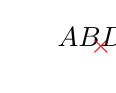
\begin{tikzpicture}[scale=1.45]
        \Tree
    [.O
    [.$A$ 
    [.$B$  [.\node[red]{$\times$}; [.$D$ ] [.$\bar D$ ] ] [.\node[red]{146}; [.$D$ ] [.$\bar D$ ] ] ] 
    [.$\bar B$  [.\node[red]{171}; [.$D$ ] [.$\bar D$ ] ] [.\node[red]{106}; [.$D$ ] [.$\bar D$ ] ] ] ]
    [.\node[red]{155}; 
    [.$B$ [.$C$ [.$D$ ] [.$\bar D$ ] ] [.$\bar C$ [.$D$ ] [.$\bar D$ ] ] ] 
    [.$\bar B$ [.$C$ [.$D$ ] [.$\bar D$ ] ] [.$\bar C$ [.$D$ ] [.$\bar D$ ] ] ] ] 
    ]
    \end{tikzpicture}
    }
    \only<6>{
      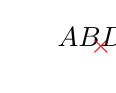
\begin{tikzpicture}[scale=1.45]
        \Tree
    [.O
    [.$A$ 
    [.$B$  [.\node[red]{$\times$}; [.$D$ ] [.$\bar D$ ] ] [.\node[red]{146}; [.$D$ ] [.$\bar D$ ] ] ] 
    [.$\bar B$  [.$C$ [.\node[red]{$\times$}; ] [.\node[red]{161}; ] ] [.\node[red]{106}; [.$D$ ] [.$\bar D$ ] ] ] ]
    [.\node[red]{155}; 
    [.$B$ [.$C$ [.$D$ ] [.$\bar D$ ] ] [.$\bar C$ [.$D$ ] [.$\bar D$ ] ] ] 
    [.$\bar B$ [.$C$ [.$D$ ] [.$\bar D$ ] ] [.$\bar C$ [.$D$ ] [.$\bar D$ ] ] ] ] 
    ]
    \end{tikzpicture}
    }
    \end{center}
\end{frame}
